\documentclass[9pt]{beamer}
\usepackage[utf8]{inputenc}
\usepackage[T1]{fontenc}
%\usepackage{verdana} %?
\usepackage[russian]{babel}
\usepackage{graphicx}
\usepackage{tikz}
\usepackage{pifont}
\usepackage{amsmath}
\usepackage{color}
\usepackage{bm}
\usepackage{amsfonts}
\usepackage{amssymb}
\usepackage{calrsfs}
\usepackage{mathtools}
\usetheme{Warsaw}
\usepackage{chronology}
\usepackage{booktabs}
\usepackage{dcolumn}

\usecolortheme{orchid}
\setbeamertemplate{frametitle}
{
    \begin{beamercolorbox}[sep=0.3cm,ht=2.2em,wd=\paperwidth]{frametitle}
        \vbox{}\vskip-2.0ex%
        \strut\insertframetitle\strut
        \vskip-0.8ex%
    \end{beamercolorbox}
}

%\renewcommand{\familydefault}{verdana}
\setbeamerfont{block title}{size=\normalsize}
\title[World development indicators]{\huge World development indicators}
\subtitle[Which country will develop more]{\large Which country will develop more}
\author[Moawad, Comandini, Isaeva, Schiavon, Snesarevskii] {{\Large Group 12:\\}Stefano Moawad\\Leonardo Comandini\\Diana Isaeva\\Andrea Schiavon\\Viktor Snesarevskii}
\date{April-May 2017}
\usebackgroundtemplate{\tikz\node[opacity=0.3] {\vbox to \paperheight{\vfil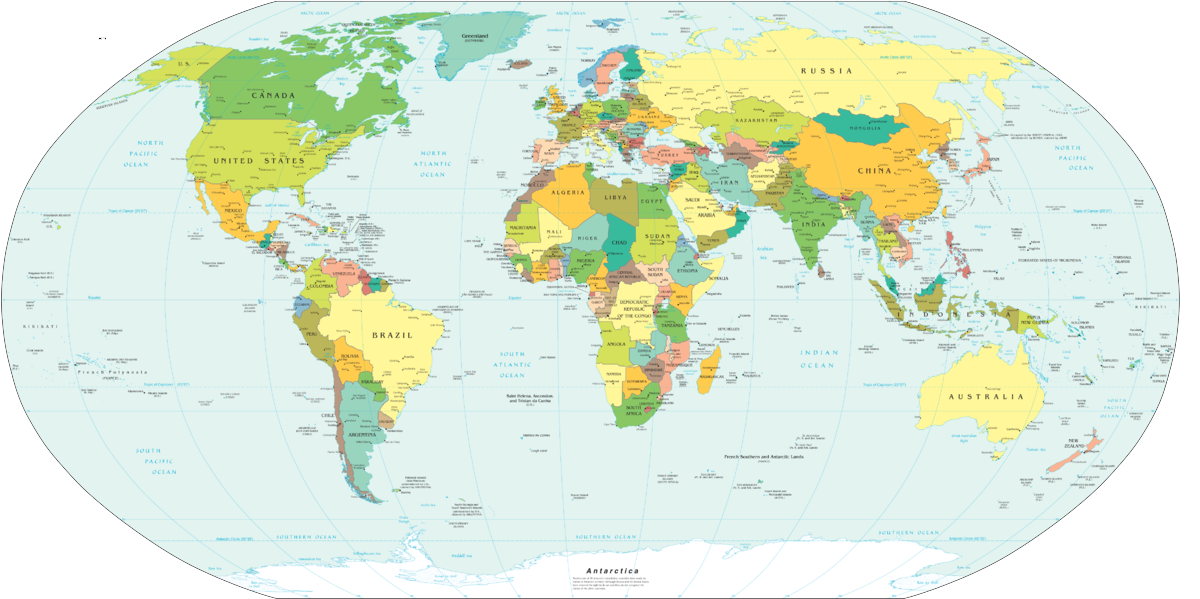
\includegraphics[width=\paperwidth]{map}\vfil}};}




\setbeamertemplate{headline}{}
\begin{document}
	\begin{frame}
	\titlepage
	\vfill
	\begin{flushright}
		
\includegraphics[height=.7cm]{kaggle.png}\quad
		
\includegraphics[height=.7cm]{worldbank.jpg}
	\end{flushright}
\end{frame}

% slide con tabella dei contenuti
\begin{frame}
	\frametitle{Table of Contents}
	\tableofcontents
\end{frame}


\section{Empirical evidences}

\begin{frame}{10-year-Growth definition and average}
	\begin{block}{}
		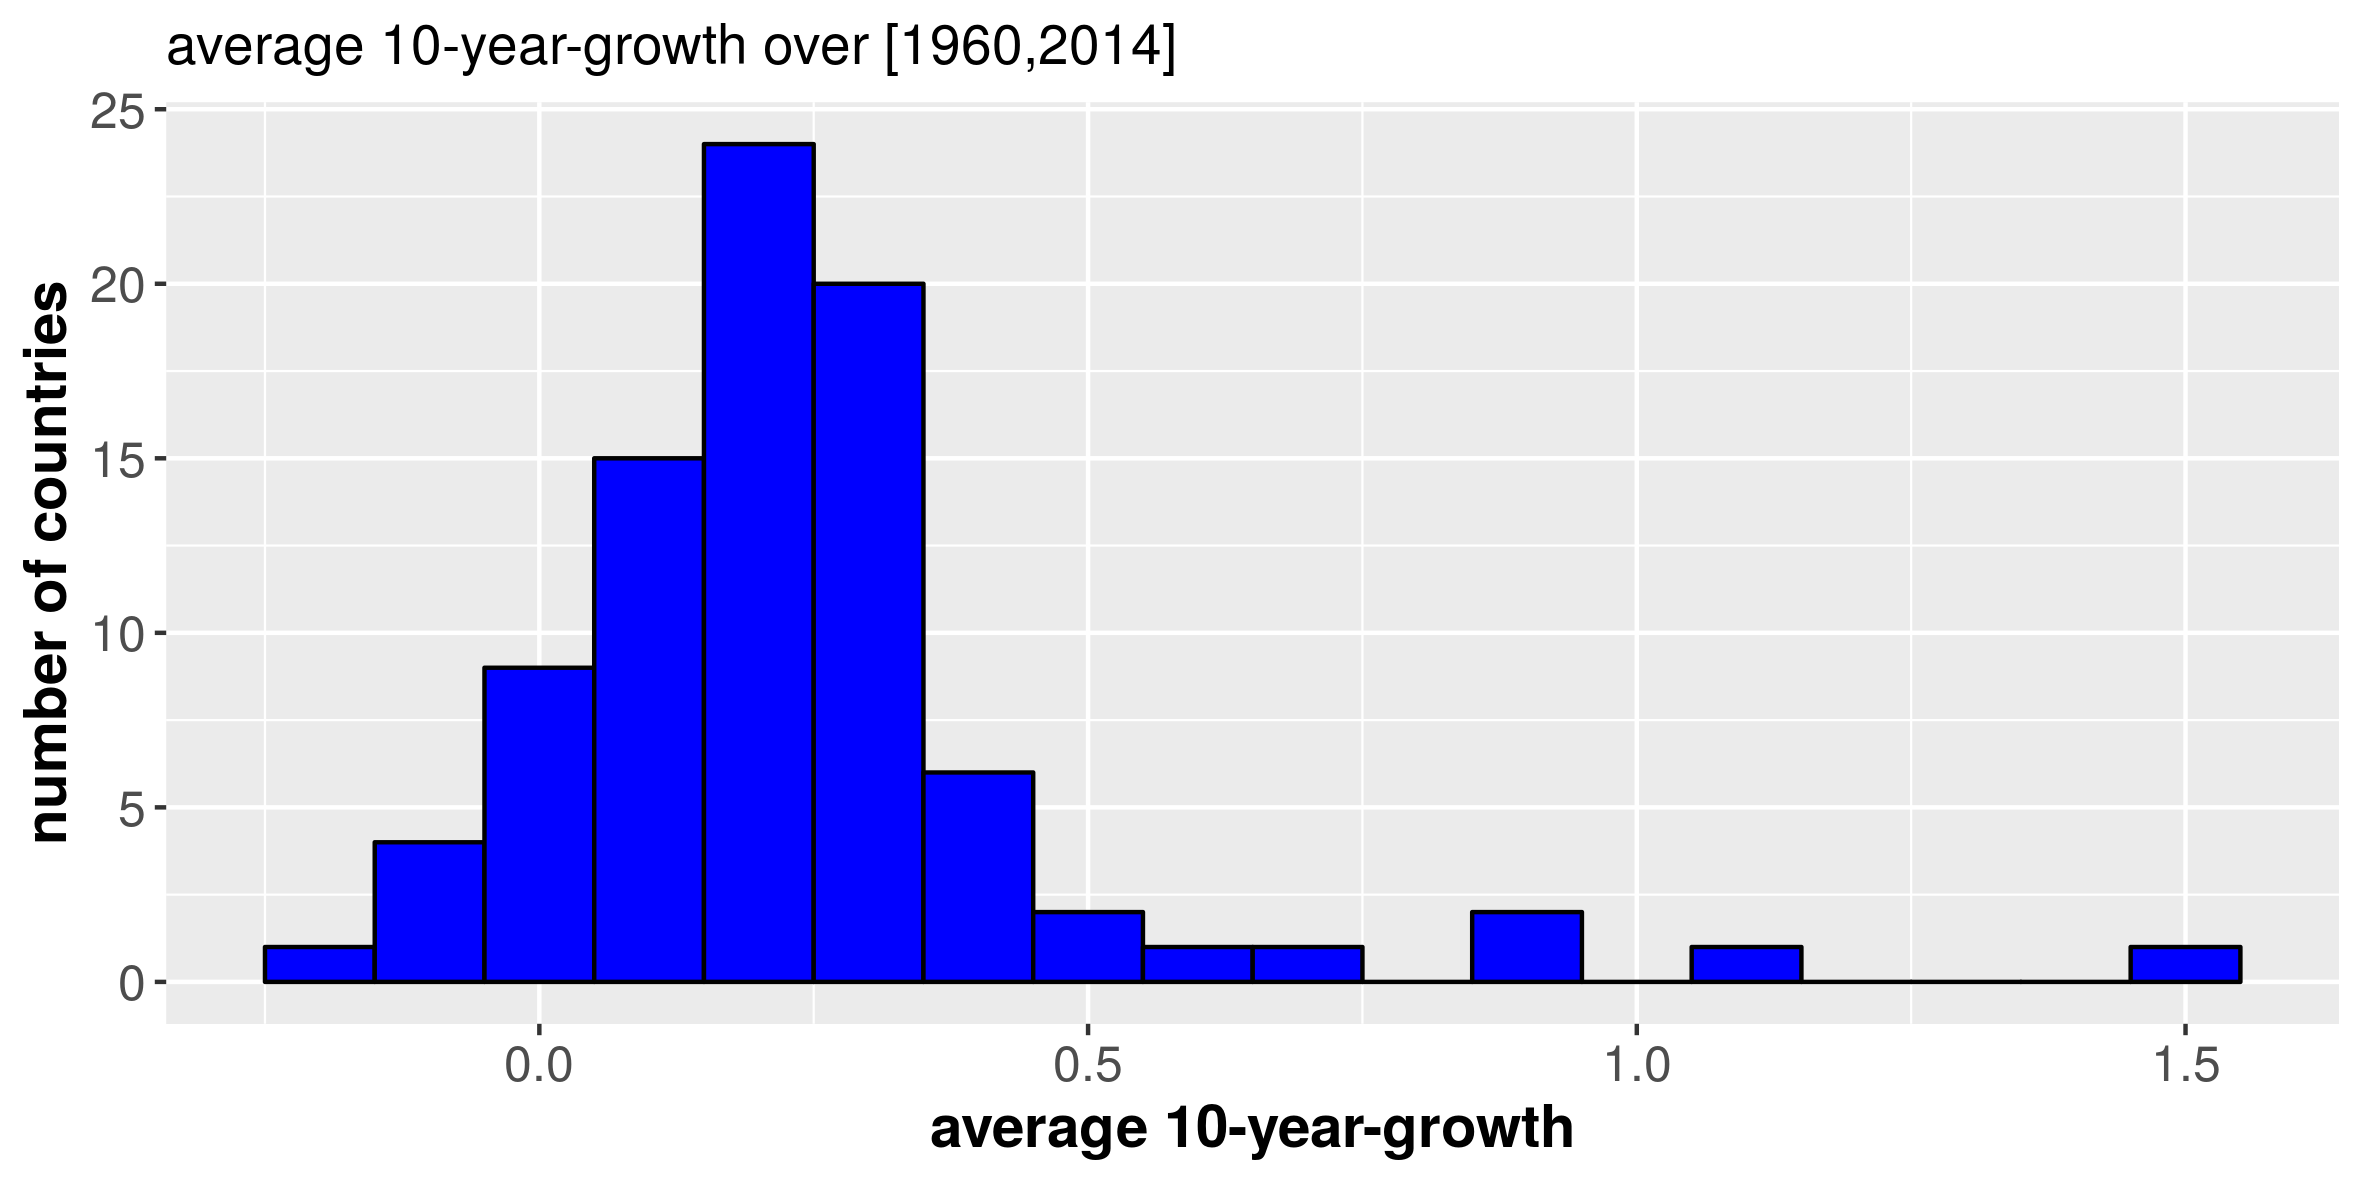
\includegraphics[height=4.5cm,width=10cm]{growth_hist.png}
	\end{block}
	\begin{block}{Definition}
		 The \alert{10-year-Growth} is the 10-year percentage variation of the GDP per capita in local currency. More formally,
		\begin{equation}
		Growth_{t} := \frac{GDP_{t}-GDP_{t-10}}{GDP_{t-10}}
		\end{equation}
		where $ GDP $ is the Gross Domestic Product per capita
		
	\end{block}
\end{frame}

\begin{frame}{10-year-growth by region}
	\begin{block}{}<1-3>
		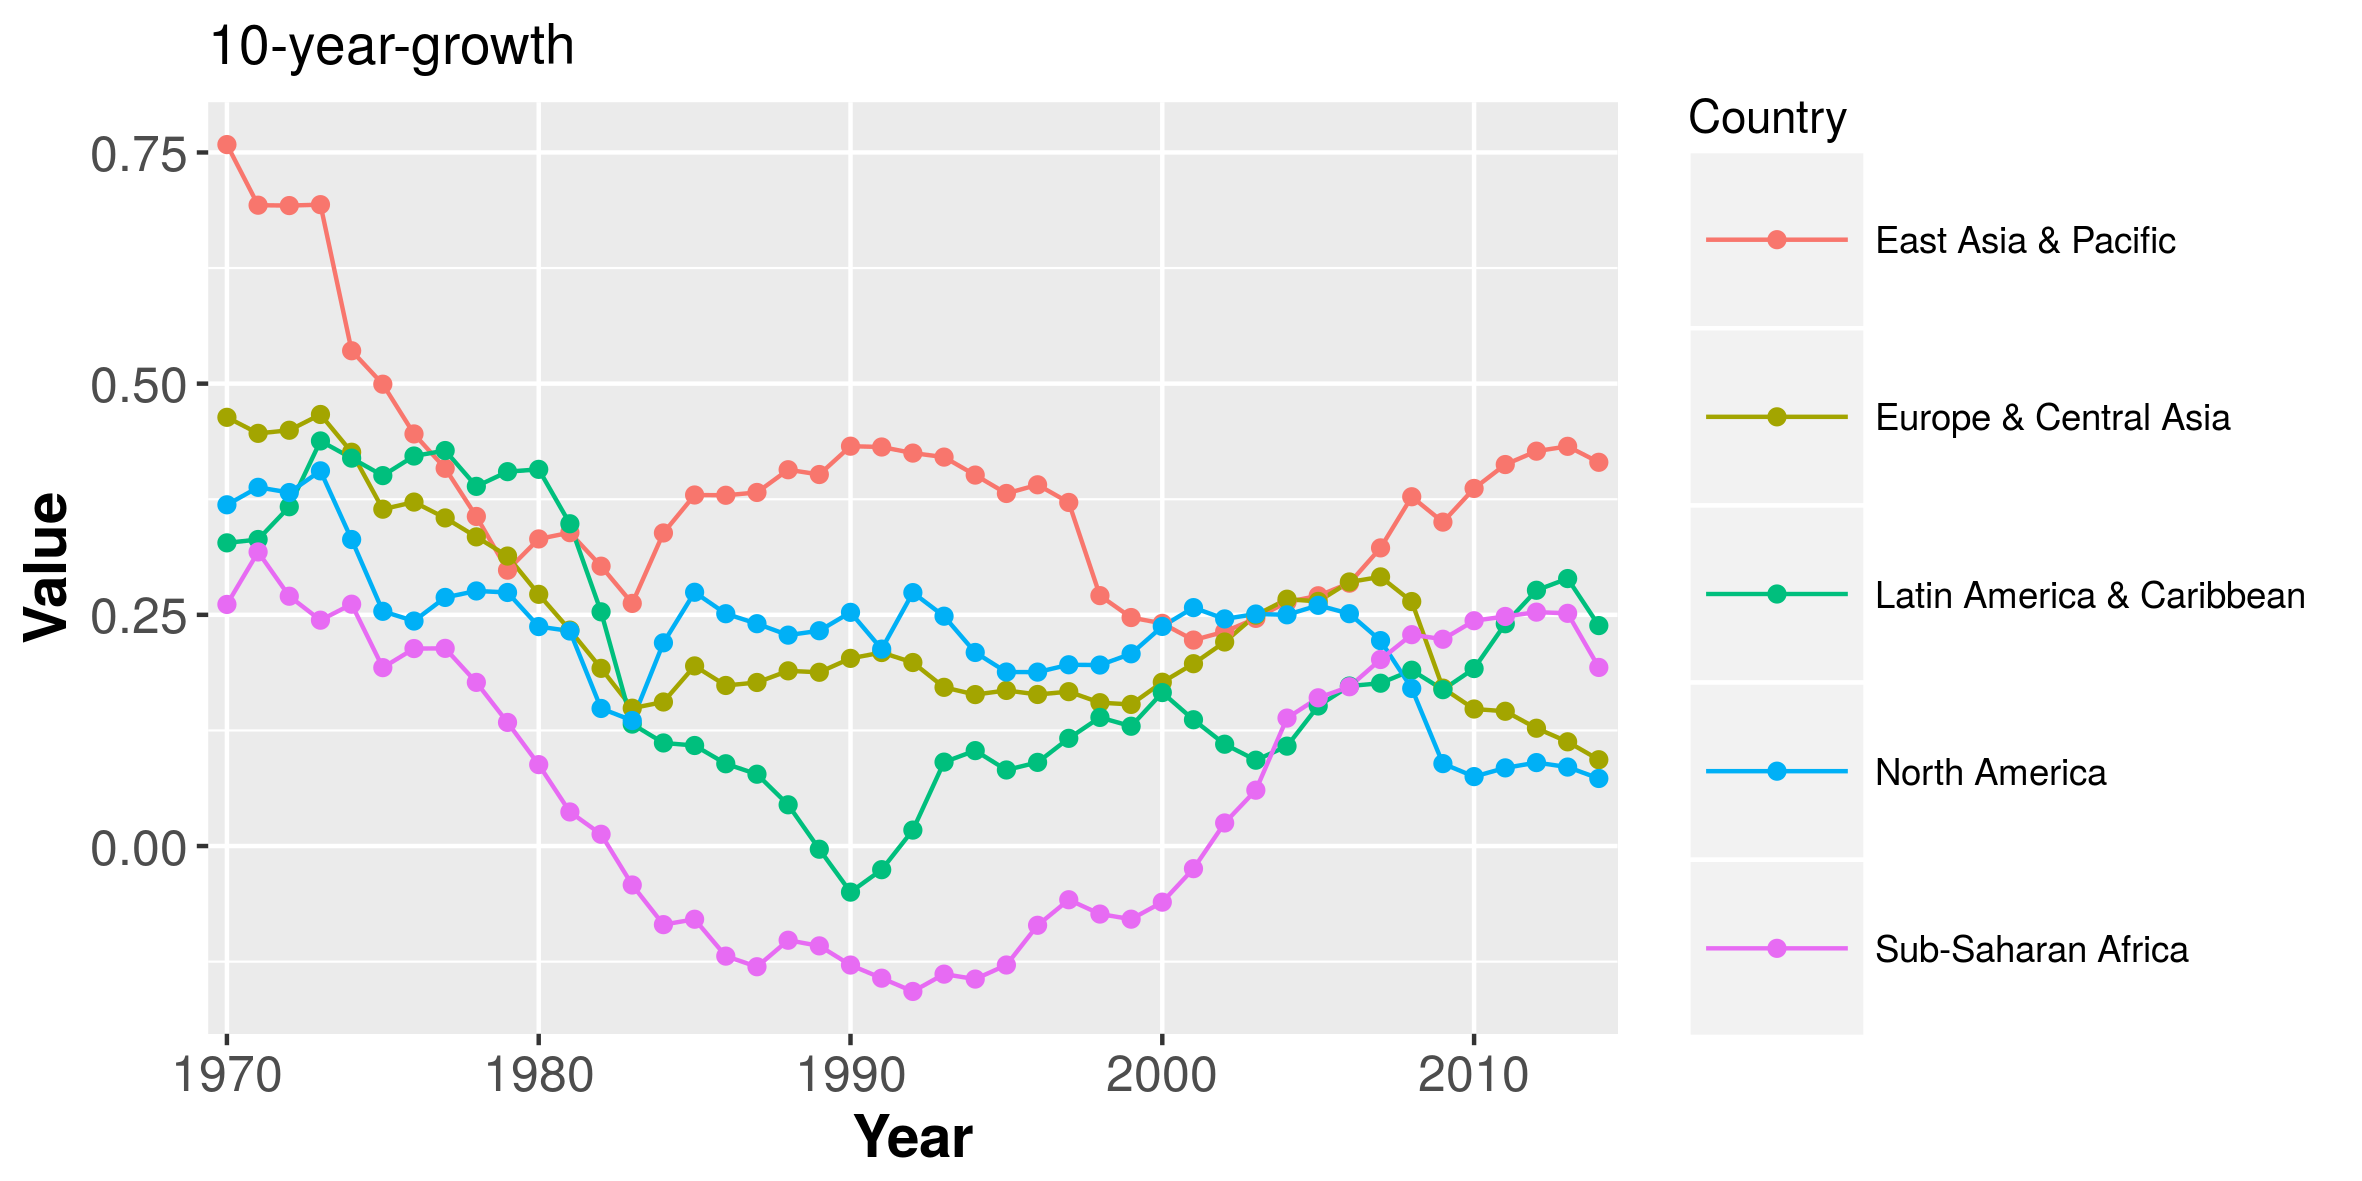
\includegraphics[height=4.5cm,width=10cm]{growth_region.png}
	\end{block}
	
		\begin{block}{Remark 1}<2-3>
			significant differences between decades $\implies$ dummy for decades
		\end{block}
		\begin{block}{Remark 2}<3>
			different growth patterns for different regions $\implies$ dummy for Asia and dummy for Africa
		\end{block}
		

\end{frame}

\begin{frame}{10-year-growth by Income group}
	\begin{block}{}
		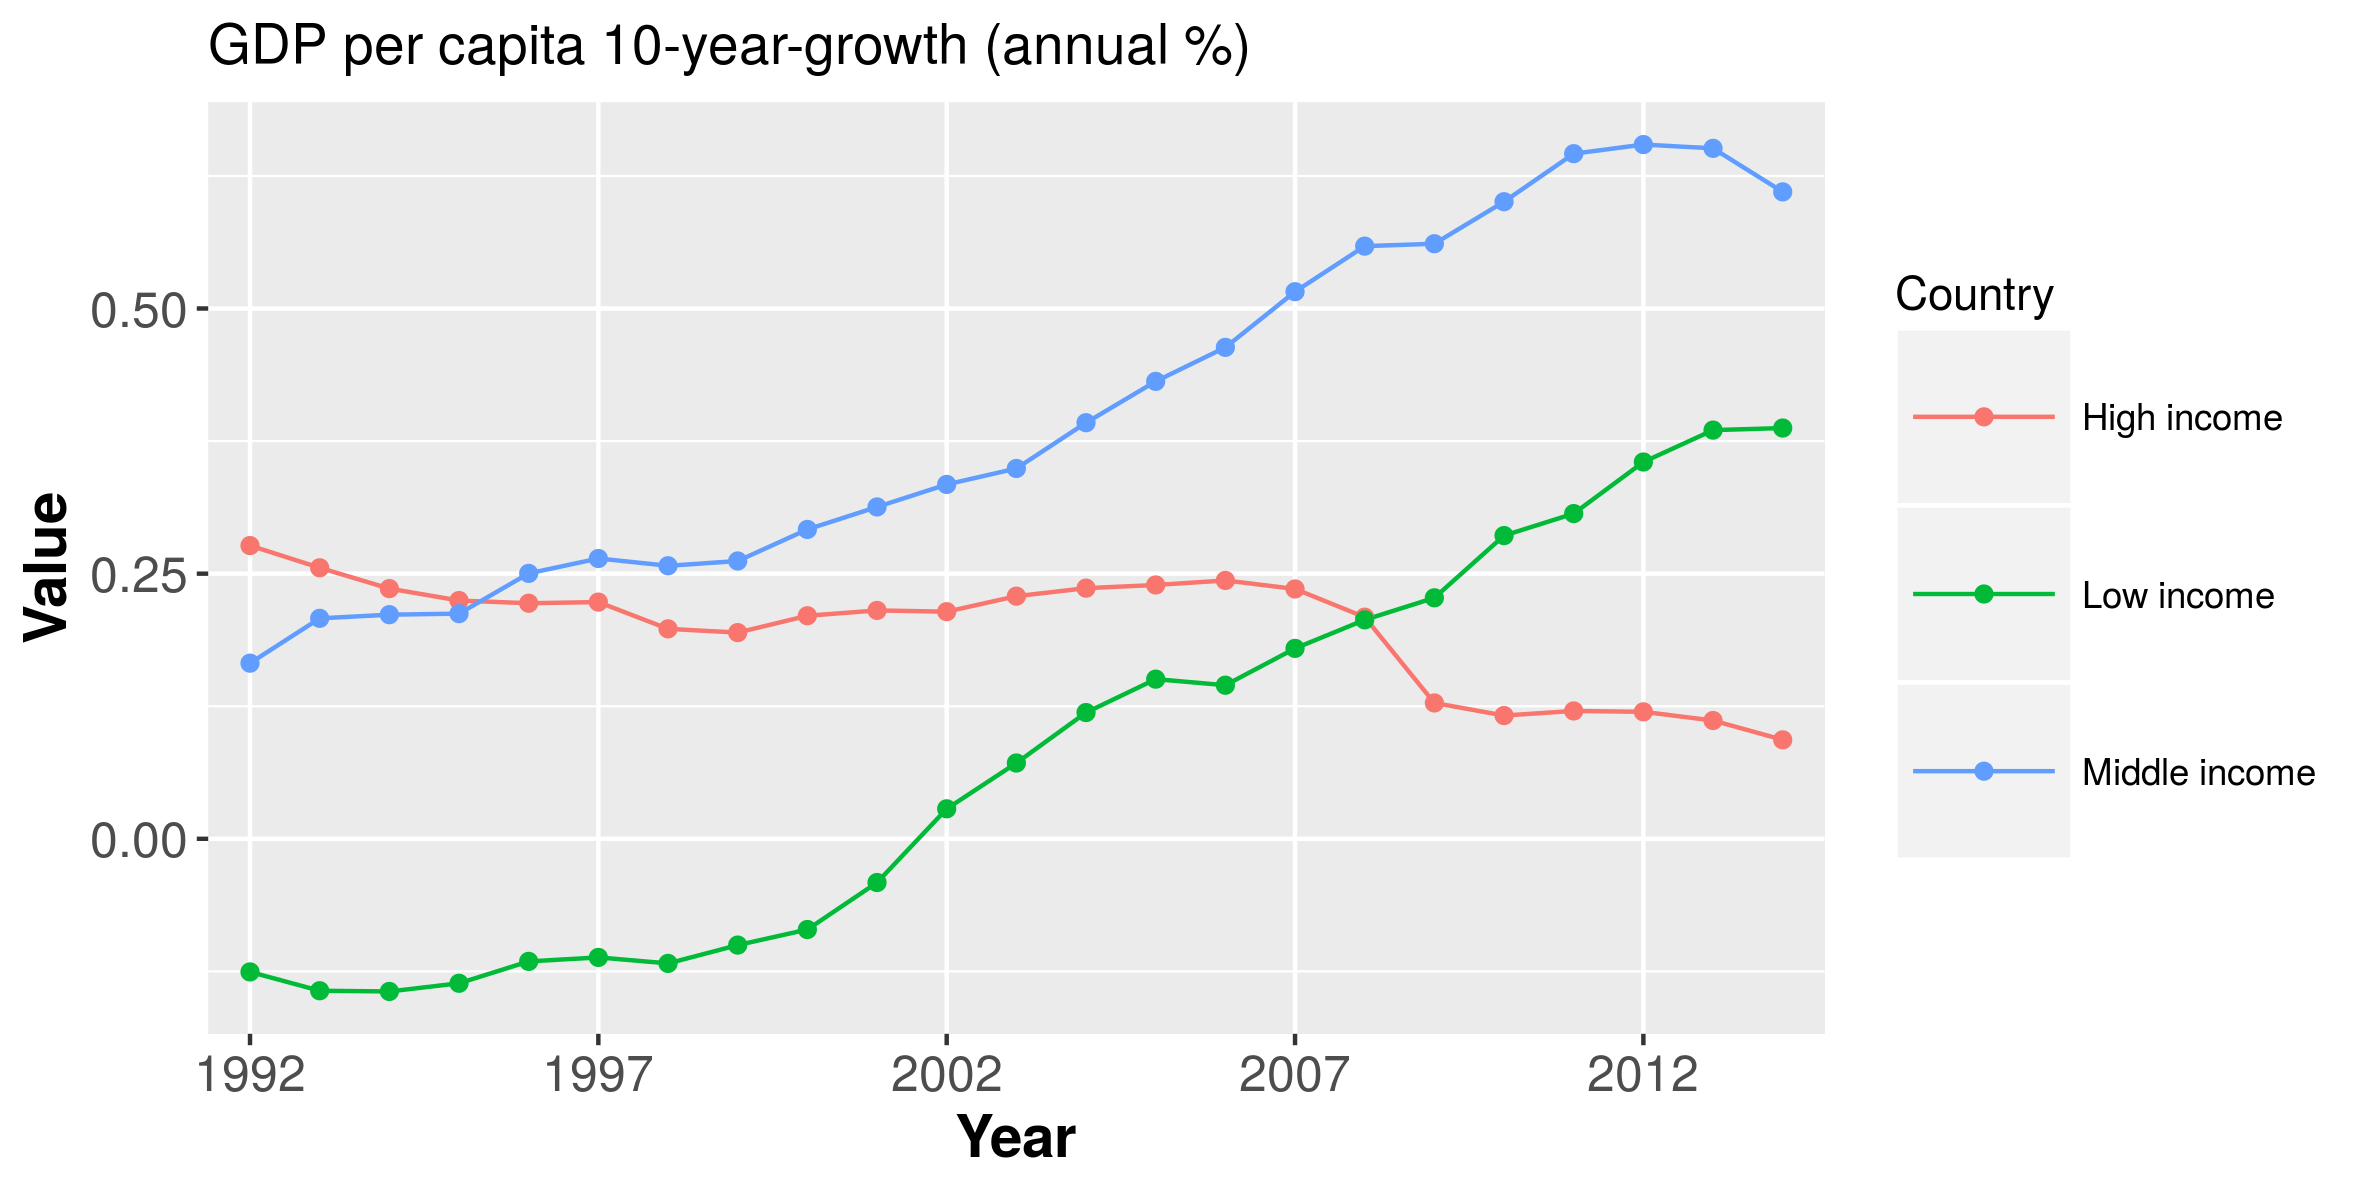
\includegraphics[height=4.5cm,width=10cm]{growth_income.png}
	\end{block}
	\begin{block}{Remark 3}
		different growth patterns for different Income groups $\implies$ dummy for High Income and dummy for Low Income
	\end{block}
\end{frame}




\section{Explanatory model for 10-year-Growth}

\begin{frame}{The Regressors: State and Environmental variables}
	\begin{block}<1-2>{State variables}
		\begin{itemize}
			\item  Education := $\frac{\text{tot enrolment primary school}}{\text{population}} \quad [\%]$
			\item Health := $\frac{1}{\text{life expectancy at birth}} \quad [\text{year}]^{-1}$
			\item Fertility := $\text{average number of births per woman}$
		\end{itemize}
		
	\end{block}
	\begin{block}<2>{Envirnonmental variables}
		\begin{itemize}
			\item Inflation [\%]
			\item GDP := $ \log(\text{GDP}) $
			\item FDI := $\text{financial capital owned by foreign investors} \quad [\% \enskip   \text{of GDP}]$
			\item Openess := $\frac{\text{Inport} + \text{Export}}{\text{GDP}}$
			\item Consumption := $\text{households consumption expenditure} \quad [\% \enskip   \text{of GDP}] $

			\item Investment := $\text{government expenditures for goods and} \newline \hspace*{2cm}\text{ services} \quad [\% \enskip   \text{of GDP}]$
		\end{itemize}
	\end{block}
\end{frame}

\begin{frame}{The Dummies: decade, income and region}
	Let ${X} = \left[\underline{x}_1,\underline{x}_2,\ldots,\underline{x}_{3n} \right]^T$ be the design matrix
	\begin{block}<1-3>{Dummies for decades}
		\begin{equation}
		D_1 = 
		\begin{cases} 
		1 & \text{if } \underline{x}_i \in [1983,1993) \\
		0       & \text{otherwise}
		\end{cases}
		\qquad
		D_2 = 
		\begin{cases} 
		1 & \text{if } \underline{x}_i \in [1993,2003) \\
		0       & \text{otherwise}
		\end{cases}
		\end{equation}
	\end{block}
	\begin{block}<2-3>{Dummies for Income}
		\begin{equation}
		I_1 = 
		\begin{cases} 
		1 & \text{if } \underline{x}_i \in \text{High Income} \\
		0       & \text{otherwise}
		\end{cases}
		\qquad
		I_2 = 
		\begin{cases} 
		1 & \text{if } \underline{x}_i \in \text{Low Income} \\
		0       & \text{otherwise}
		\end{cases}
		\end{equation}
	\end{block}
	\begin{block}<3>{Dummies for Region}
		\begin{equation}
		R_1 = 
		\begin{cases} 
		1 & \text{if } \underline{x}_i \in \text{East Asia} \\
		0       & \text{otherwise}
		\end{cases}
		\qquad
		R_2 = 
		\begin{cases} 
		1 & \text{if } \underline{x}_i \in \text{Sub-Saharan Africa} \\
		0       & \text{otherwise}
		\end{cases}
		\end{equation}
	\end{block}
\end{frame}

\begin{frame}{Linear Model: complete model}
	Let $ \epsilon \sim N(0,\sigma^2)$
	\begin{block}{complete model}
		\begin{align*}
		Growth &= \beta_0+\beta_1\text{fertility}+\beta_2\text{FDI}+\beta_3\text{GDP}+\beta_4\text{education}+\beta_5\text{consumption}+\\
		&\qquad \beta_6\text{inflation}+\beta_7\text{health}+\beta_8\text{investment}+\beta_9\text{openess}+\\
		& \qquad \beta_{10}D_1+\beta_{11}D_2+\beta_{12}R_1+\beta_{13}R_2+\beta_{14}I_1+\beta_{15}I_2+\\
		&\qquad D_1(\beta_{16}\text{GDP}+\beta_{17}\text{fertility}+\beta_{18}\text{investment})+\\
		&\qquad D_2(\beta_{19}\text{GDP}+\beta_{20}\text{fertility}+\beta_{21}\text{investment})+\\
		&\qquad I_1(\beta_{22}\text{GDP}+\beta_{23}\text{fertility}+\beta_{24}\text{investment})+\\
		&\qquad I_2(\beta_{25}\text{GDP}+\beta_{26}\text{fertility}+\beta_{27}\text{investment})+\\
		&\qquad R_1(\beta_{28}\text{GDP}+\beta_{29}\text{fertility}+\beta_{30}\text{investment})+\\
		&\qquad R_2(\beta_{31}\text{GDP}+\beta_{32}\text{fertility}+\beta_{33}\text{investment}) + \epsilon \end{align*}
	\end{block}
\end{frame}
\begin{frame}{Linear Model: reduced model}
	Let $ \epsilon \sim N(0,\sigma^2)$
    \begin{block}{reduced model}
    	\begin{align*}
    	Growth &= \beta_0+\beta_1\text{fertility}+\beta_2\text{GDP}+\beta_3\text{consumption}+\beta_4\text{investment}+\\
    	&\qquad \beta_{5}\text{education}+\beta_{6}\text{FDI}\\
    	& \qquad \beta_{7}D_1+\beta_{8}D_2+\beta_{9}R_1+\beta_{10}R_2+\beta_{11}I_1+\beta_{12}I_2+\\
    	& \qquad D_1(\beta_{13}\text{GDP}+\beta_{14}\text{investment})+\\
    	& \qquad
    	 D_2(\beta_{15}\text{GDP})+\\
    	& \qquad I_1(\beta_{16}\text{GDP}+\beta_{17}\text{fertility}+\beta_{18}\text{investment})\\
    	& \qquad I_2(\beta_{19}\text{investment}) +\\
    	&\qquad R_1(\beta_{20}\text{GDP}+\beta_{21}\text{fertility})+\\
    	&\qquad
    	R_2(\beta_{22}\text{fertility}+\beta_{23}\text{investment}) + \epsilon \end{align*}
    \end{block}
   
\end{frame}
\begin{frame}{lm output}
	\begin{columns}[T] 
		\begin{column}[T]{5cm}
			\begin{tabular}{l D{)}{)}{17)3} }
				\toprule
				& \multicolumn{1}{c}{Model 1} \\
				\midrule
				(Intercept)   & 0.9531 \; (0.3791)^{*}    \\
				fertility     & -0.0849 \; (0.0244)^{***} \\
				FDI           & -0.0085 \; (0.0063)       \\
				GDP           & \textcolor{red}{-0.0903} \; (0.0305)^{**}  \\
				education     & -0.0025 \; (0.0010)^{*}   \\
				consumption       & 0.0047 \; (0.0010)^{***}  \\
				health        & -21.0428 \; (11.8102)     \\
				R1            & 3.8459 \; (0.3718)^{***}  \\
				R2            & 0.8626 \; (0.1585)^{***}  \\
				I1            & 1.0546 \; (0.4503)^{*}    \\
				I2            & -0.4912 \; (0.1445)^{**}  \\
				investment    & 0.0407 \; (0.0063)^{***}  \\
				D1            & -0.3408 \; (0.1521)^{*}   \\
				D2            & -0.4913 \; (0.1369)^{***} \\
				GDP:D1        & 0.0841 \; (0.0182)^{***}  \\
				investment:D1 & -0.0189 \; (0.0048)^{***} \\
				GDP:D2        & 0.0640 \; (0.0163)^{***}  \\
				GDP:I1        & -0.0783 \; (0.0474)       
				
			\end{tabular}
		\end{column}
		\begin{column}[T]{5cm} 
			\begin{tabular}{l D{)}{)}{17)3} }
				\toprule
				& \multicolumn{1}{c}{} \\
				\midrule
				fertility:I1  & 0.0804 \; (0.0297)^{**}   \\
				investment:I1 & -0.0354 \; (0.0073)^{***} \\
				investment:I2 & 0.0327 \; (0.0088)^{***}  \\
				GDP:R1        & -0.3070 \; (0.0348)^{***} \\
				fertility:R1  & -0.3880 \; (0.0362)^{***} \\
				fertility:R2  & -0.0527 \; (0.0274)       \\
				investment:R2 & -0.0425 \; (0.0073)^{***} \\
				\midrule
				R$^2$         & 0.8705                    \\
				Adj. R$^2$    & \textcolor{red}{0.8364}                   \\
				Num. obs.     & 116                       \\
				RMSE          & 0.1134                    \\
				\bottomrule
				\multicolumn{2}{l}{\scriptsize{$^{***}p<0.001$, $^{**}p<0.01$, $^*p<0.05$}}
			\end{tabular}
			{\footnotesize  
				 Legend:\begin{itemize}
					\item D1 = [1983,1993) \enskip D2 = [1993,2003)
					\item R1 = Asia \enskip R2 = Africa
					\item I1 = high income
					\item I2 = low income
					
				\end{itemize}
			}
			
		\end{column}
	\end{columns}
\end{frame}

\begin{frame}{Results analysis: Conditional Convergence}
	
	\begin{block}{}
		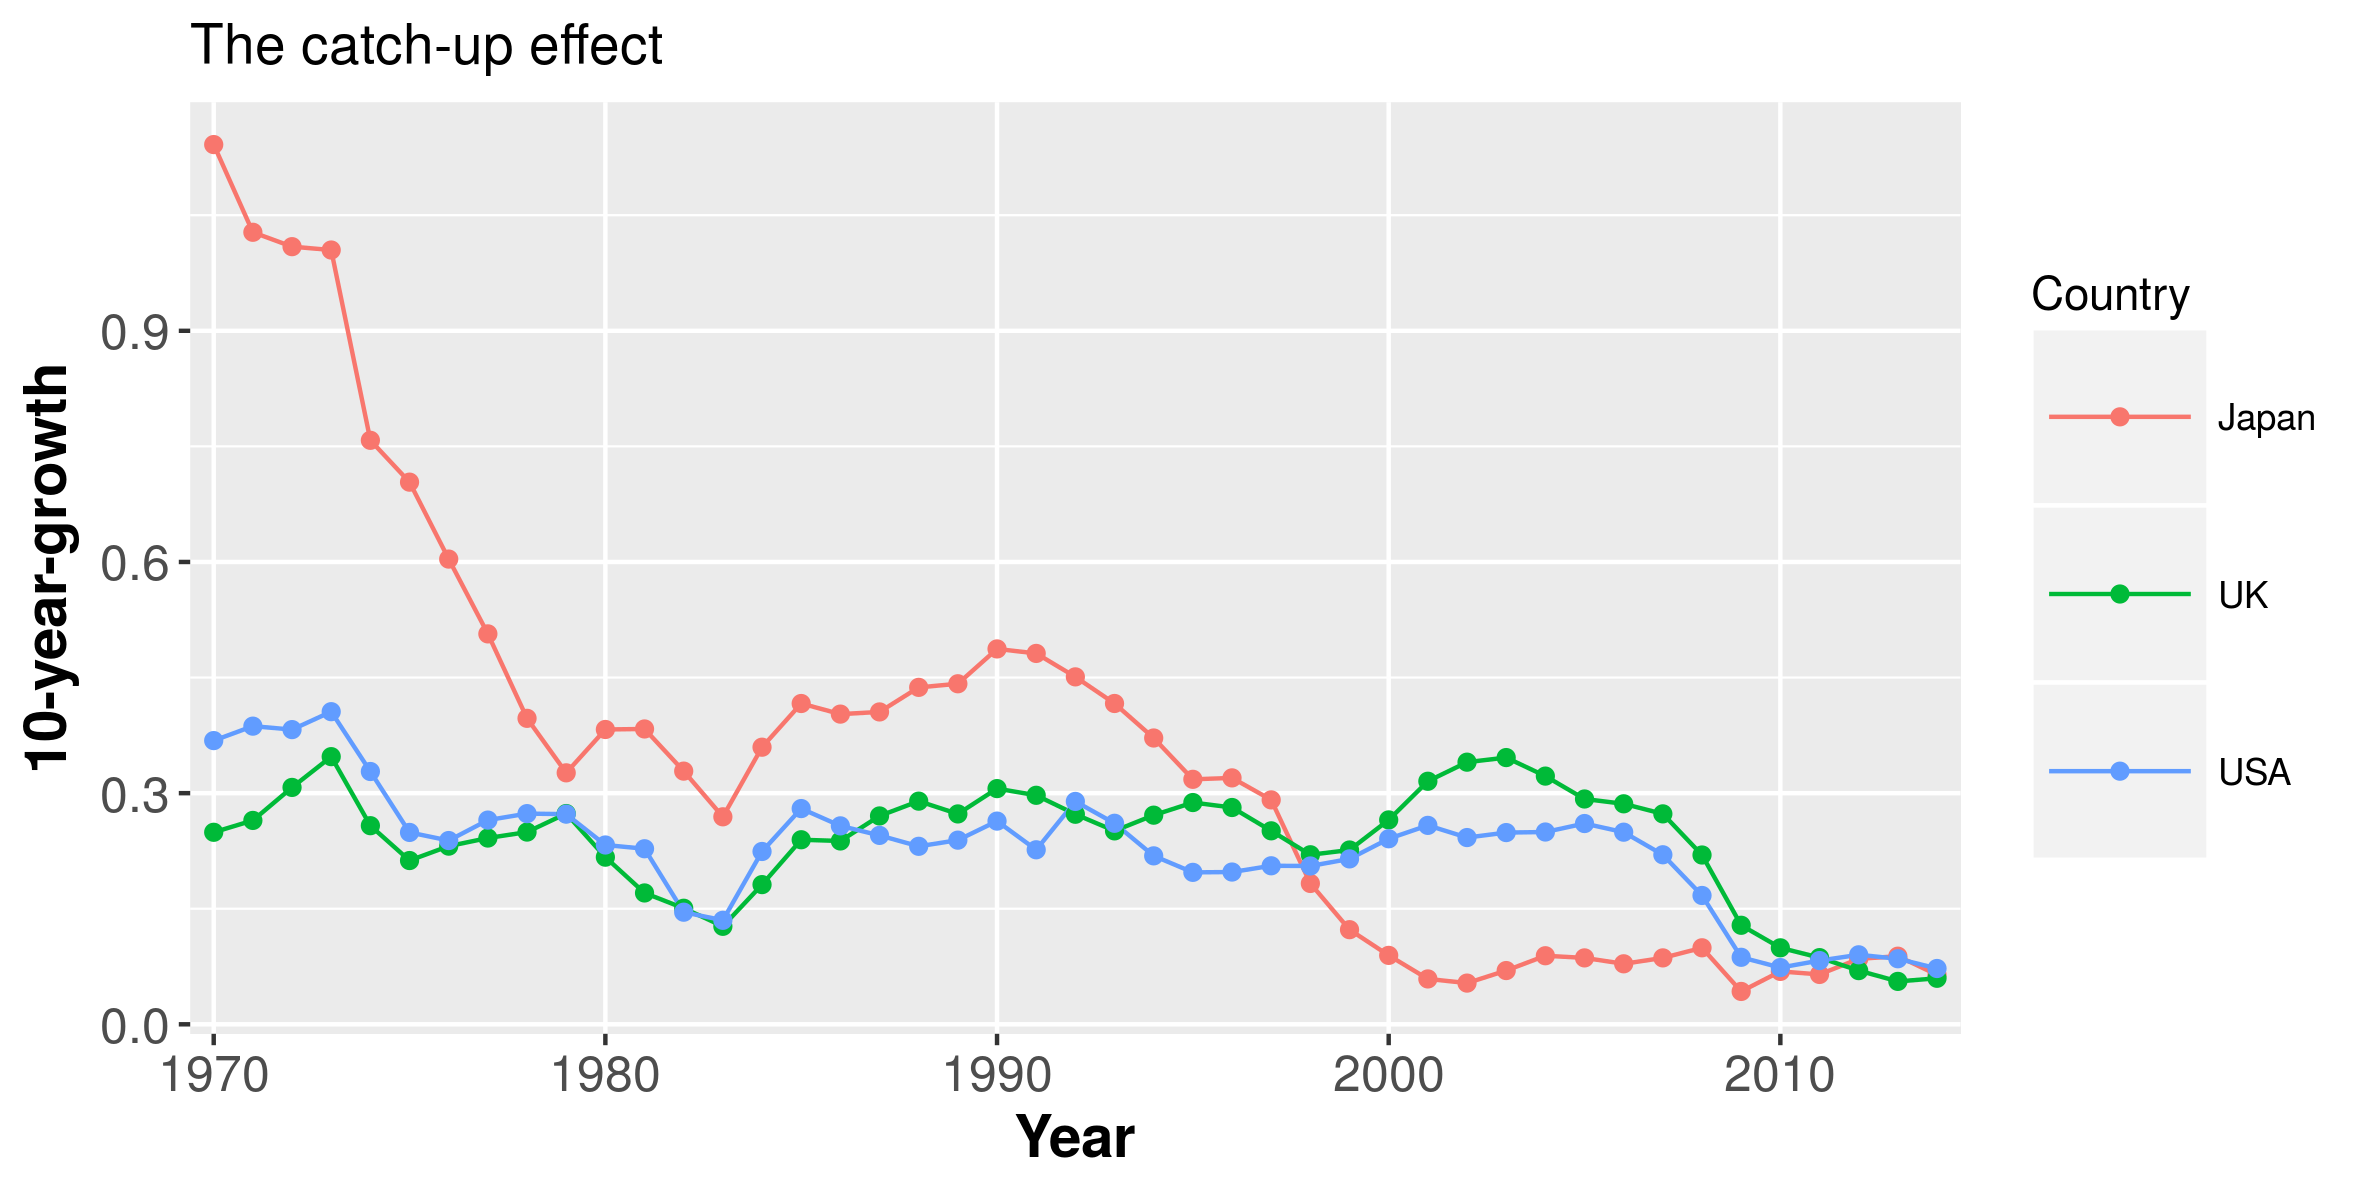
\includegraphics[height=4.5cm,width=10cm]{convergence.png}
	\end{block}
	\begin{definition}
		the following principle is called \textbf{conditional convergence}: the lower the initial GDP the higher the growth over the next decade
	\end{definition}
			
\end{frame}


\section{Prediction, Evaluation and Comparison}

\begin{frame}{Prediction model: no dummies for decades}
	Let $ \epsilon \sim N(0,\sigma^2)$
	\begin{block}{prediction model: timeless}
		\begin{align*}
		Growth &= \beta_0+\beta_1\text{fertility}+\beta_2\text{GDP}+\beta_3\text{consumption}+\beta_4\text{investment}+\\
		& \qquad 
		\beta_5R_1+\beta_{6}R_2+\beta_{7}I_1+\beta_{8}I_2+\\
		& \qquad
        I_1(\beta_{9}\text{GDP}+\beta_{10}\text{fertility}+\beta_{11}\text{investment})\\
		& \qquad 
		I_2(\beta_{12}\text{investment} + \beta_{13}\text{fertility}) +\\
		&\qquad R_1(\beta_{14}\text{GDP}+\beta_{15}\text{fertility})+\\
		&\qquad
		R_2(\beta_{16}\text{fertility}+\beta_{17}\text{investment}) + \epsilon \end{align*}
	\end{block}
\end{frame}

\begin{frame}{predictor evaluation}
	fitting sample = [1983,2003] \qquad test sample = [2003,2013]
	\begin{definition}<1-2>
		\begin{itemize}
			\item $F_t =$ prediction for the growth in $t$ with our model
			\item $Y_t =$ realization of growth in $t$
			\item $e_t =$ prediction error
			\item $ME = \sum_{t=0}^{n}\frac{1}{n}e_t =$ mean error 
			\item $MAD = \sum_{t=0}^{n}\frac{1}{n}\|e_t\| = $ mean absolute deviation 
			\item $ RMSE = \sqrt{\sum_{t=0}^{n}\frac{1}{n}e_t^{2} =}$ root mean square error
		\end{itemize}
		
	\end{definition}
	\begin{block}<2>{predictor performances}
	\begin{columns}
		\begin{column}{5cm}
		\begin{tabular}{ r|c|c| }
			\multicolumn{1}{r}{}
			&  \multicolumn{1}{c}{same countries}
			& \multicolumn{1}{c}{new countries} \\
			\cline{2-3}
			ME & -0.014 & 0.022 \\
			\cline{2-3}
			MAD & 0.099 & 0.182 \\
			\cline{2-3}
			RMSE & 0.1361 & 0.2823 \\
			\cline{2-3}
		\end{tabular}
	\end{column}
	\begin{column}{3cm}
		\begin{itemize}
			\item slightly overestimating
			\item inaccurate out-of-sample
		\end{itemize}
	\end{column}
    \end{columns}
	\end{block}	
	
	
\end{frame}

\begin{frame}{2020 growth prediction comparison}
	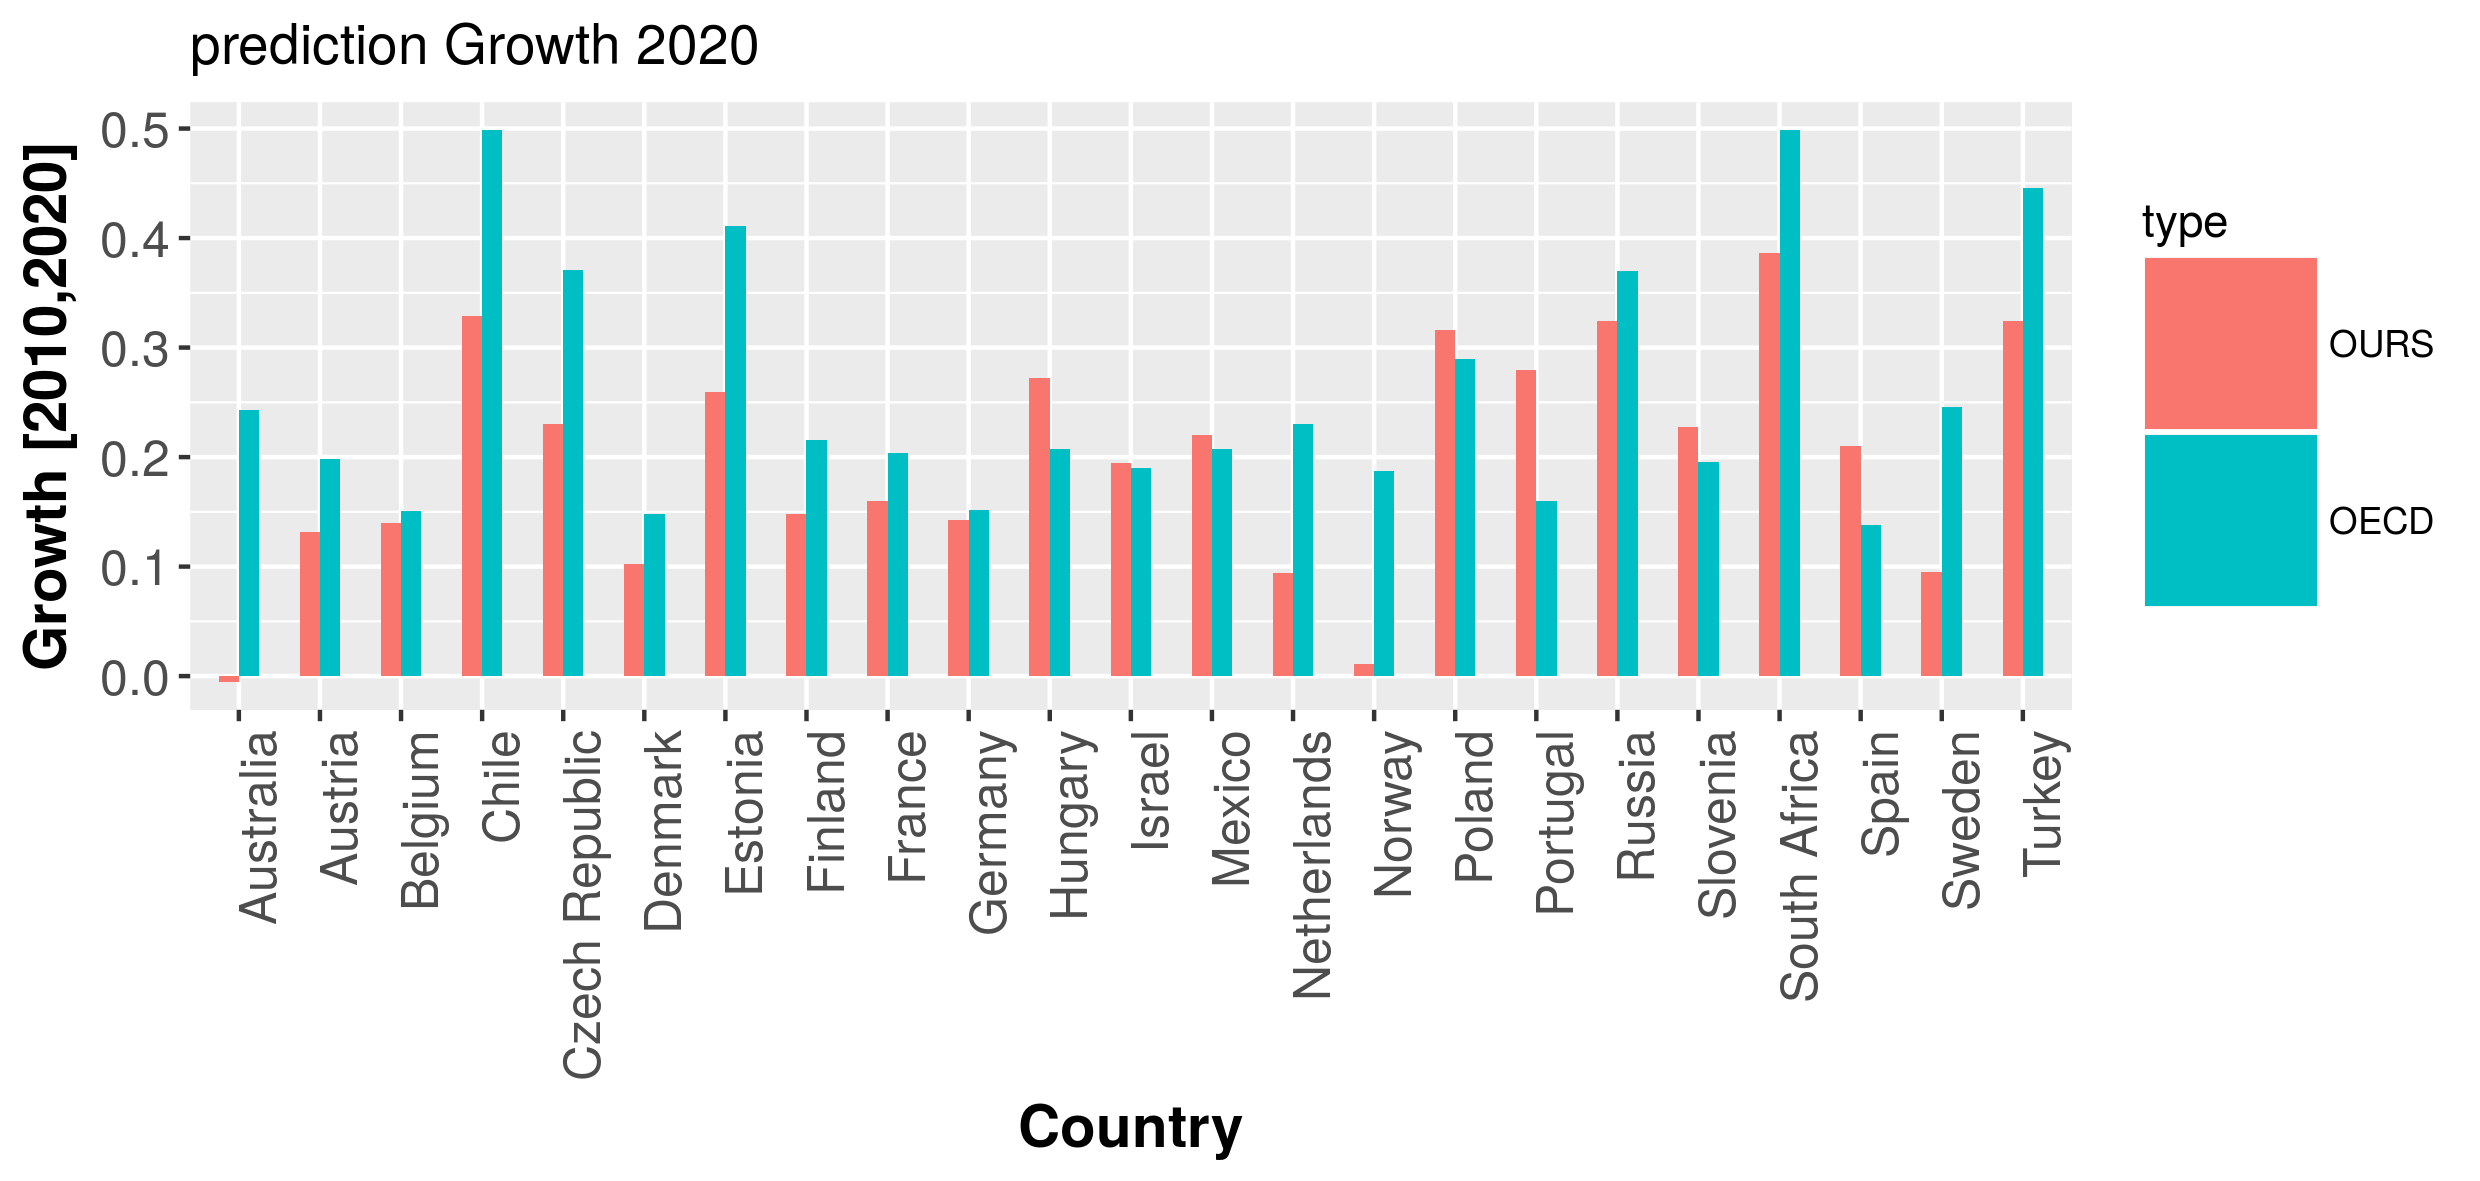
\includegraphics[height=6.5cm,width=11.5cm]{OECD.png}
	
	
	\textbf{OECD} = The Organisation for Economic Co-operation and Development  is an intergovernmental economic organisation with 35 member countries, founded in 1960 to stimulate economic progress and world trade
\end{frame}




\end{document}